\section{Klassische Enterprise-Architektur}

%%%%%%%%%%%%%%%%%%%%%%%%%% Monolith Architecture %%%%%%%%%%%%%%%%%%%%%%%%%%%

\begin{frame}{Monolith Architecture}
    \begin{itemize}
        \item Monolith ist altgriechisch für \textit{einheitlicher Stein}
        \item Einheitlich: Alles ist eins - alle Funktionalitäten in einer Komponente
        \item Stein: Altes Material - früher gut. Heute schlecht?
        \item Problem: Enge Kopplung
    \end{itemize}
\end{frame}

\begin{frame}{Monolith Architecture: Beispiel E-Commerce}
    \begin{figure}[!h]
        \centering
        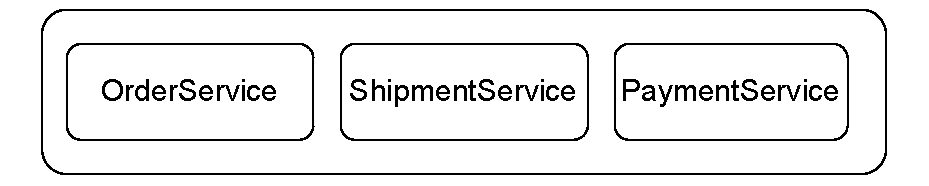
\includegraphics[scale=0.70]{imglib/mono/mono}
        \caption{E-Commerce-Beispiel mit Monolith Architecture}
        \label{fig:mono-ecommerce}
    \end{figure}
\end{frame}

\begin{frame}{Monotlith Architecture: Agilität}
    \begin{itemize}
        \item Enge Kopplung ist fatal
        \begin{itemize}
            \item Keine kleinen autonomen Teams
            \item Erhöhte Komplexität und schwere Wartung $\Rightarrow$ längere Iterationen $\Rightarrow$ unflexibel
            \item Funktionalitäten nicht wiederverwendbar $\Rightarrow$ Mehraufwand \& Duplikation $\Rightarrow$ Änderungen teuer
            \item Isolierte Funktionstests sind möglicherweise aufwendig
        \end{itemize}
        \item Auslieferung nur im Ganzen \& längere Iterationen $\Rightarrow$ seltene Auslieferung
        \item Horizontale Skalierung kaum möglich
        \item Aber: System ist nicht verteilt $\Rightarrow$ Keine Intersystemkommunikation $\Rightarrow$ Geringe Time-to-Market \& möglicherweise einfache System-Tests
        \item Ideal für lokale Anwendungen ohne Skalierungsbedarf bei welchen Flexibilität nicht notwendig ist
    \end{itemize}
\end{frame}

%%%%%%%%%%%%%%%%%%%%%%%%%% Modular Monolith Architecture %%%%%%%%%%%%%%%%%%%%%%%%%%%

\begin{frame}{Modular Monolith Architecture}
    \begin{itemize}
       \item Bisher: Eng gekoppelte Komponenten mit gegenseitigen Abhängigkeiten
       \item Jetzt: Module für bessere separation of concerns
       \item Evolution monolithischen Architektur, um die Abhängigkeiten zu eliminieren
     \end{itemize}
\end{frame}

\begin{frame}{Monolith Architecture: Beispiel E-Commerce II}
    \begin{figure}[!h]
        \centering
        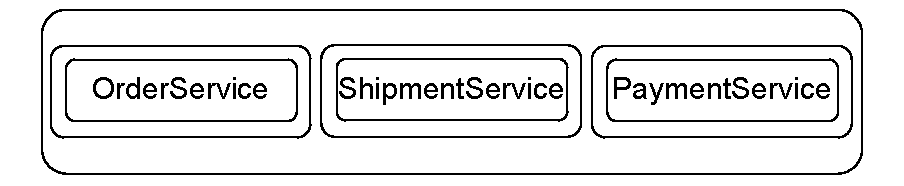
\includegraphics[scale=0.55]{imglib/mono/mono-example}
        \caption{E-Commerce-Beispiel mit Modular Monolith Architecture}
        \label{fig:mono-modular}
    \end{figure}
\end{frame}

\begin{frame}{Modular Monolith Architecture: Agilität}
    \begin{itemize}
      \item Klare Trennung der Module $\Rightarrow$ Höhe Cohesion $\Rightarrow$ kurze iterierte Release-Zyklen
      \item Änderungen in einzelnen Modulen beeinträchtigen nicht mehr das gesamte System $\Rightarrow$ Änderungen selbst spät in der Entwicklung möglich
      \item Lose Module $\Rightarrow$ einfache Testbarkeit $\Rightarrow$ Lieferung funktionierender Software
      \item Aber: Höhe Anforderungen an Entwickler $\Rightarrow$ Integration Testing und regelmäßige Review und Refactoring notwendig
    \end{itemize}
\end{frame}
